\documentclass{article}
\usepackage[utf8]{inputenc}
\usepackage[english]{babel}
\usepackage{graphicx}
\usepackage{amsmath}
\usepackage{amssymb}
\usepackage{amsfonts}
\usepackage{amsthm}
\usepackage{subcaption}


\usepackage{biblatex}
\addbibresource{./bibli.bib}
\usepackage{hyperref}
\graphicspath{ {plots/} }
\hypersetup{
	linktocpage=true,
	colorlinks=true,
	linkcolor=red,
	filecolor=magenta,      
	urlcolor=cyan,
	pdftitle={Kelly's Criterion},
	pdfpagemode=FullScreen,
	bookmarks=true,
	breaklinks=true
}

\urlstyle{same}
\newtheorem{thm}{Theorem}[section]
\newtheorem{cor}[thm]{Corollary}
\newtheorem{lem}[thm]{Lemma}
\newcommand{\pdiv}[2]{{\frac{\partial#1}{\partial#2}}}

\title{Mathematical Model's course work of Kelly's Criterion}
\date{2021-09-01}
\author{Eldad Kronfeld}


\begin{document}
	\maketitle
	\thanks{Thank you Hagai for the continuing patience and support along the way.}
	\tableofcontents
	\newpage
	\section{Introduction}
		This paper is about a mathematical model influenced by John Kelly's work\cite{6771227}  at the early 1950s explained in this book\cite{Finance}, 
		the model that I propose simulate the process of investing in stocks and gaining or losing from the investments.
		The model looks at the values of the stocks at fixed intervals of discrete times. at each time frame (which is a round of the simulation) we are presented with the ability to split our money between all of the stocks and options, meaning we can decide how much to invest in each stock, or alternately not invest at all. each stock's value can randomly change at each round, as a product of that our gains or losses are proportional to the amount of money we decided to invest in the stock.\\
		Investing in stocks using Kelly's method isn't new at all and was used by many well established investors including:
		Warren Buffett\cite{buffet} and Bill Gross\cite{wiki}.
		The model shows as that if we want to maximize our gains in the long run certain money distributions are superior to others and are expected to preform better then the rest, and untimely in each case we can find a strategy to invest our money that would be superior to all the other investment options.\\
		At the start of the paper I will define a simplified model which include one option, however the option have multiple outcomes that can accrue at each time-frame, later I will show some examples and the results from the simulation of the mode.
		At later parts I will include multiple stock options with multiple outcome each in order to fully develop the model into something a bit more realistic where we have multiple choices instead of just one.
		The model's simulation was constructed using state of the art software package in order to allow easy manipulation of the model's attributes and variable while keeping state of the art performance at all the tested problem sizes.
	\section{The Base model}
	\subsection{Defining The Model}
	The model which is  influenced by John Kelly's work \cite{Finance} runs till infinity (ideally) in discrete time frames, which I will call ticks$\backslash$rounds, however we will run at to around $100-500$ rounds each run.
	\newline
	One the Hypothesis of the model is that the investments or gambles we take each round have expectations that are greater then 1,
	\begin{equation}
		\label{Expected}
	 E_{gain} \ge 1		
	\end{equation}
	\\
	Meaning that in the long run we can expect that we will yield revenue from the ventures and not loss from it however because of the random nature of the model losses can happen and even at some cases total ruin.
	\newline
	If we define a simple model, where we have one stock with $k$ possible outcomes, where each outcome has $p_i$ probability of happening, and we invest a fraction $f$ of our money and keep the rest which is $b=1-f$ 
	\begin{equation}
		\label{nes}
		F_N = \Bigg\{
		\begin{aligned}
			&(b + f\cdot \gamma _i)F_{N-1} &&N>1 \text{, for }i=1,..,k \\
			&1 &&for \enspace N=0
		\end{aligned}
	\end{equation}
	\\
	Throughout all of the explanations and simulations I will normalize the results to be such as that we start with 1$\textdollar$ and each hypocritical return will be noted as $\gamma_i\cdot F_{N-1}$, where $F_{N-1}$ denotes the sum of money from round $N-1$ and $\gamma$ denotes the gain and $\gamma\in[0,\infty)$, so when $\gamma = 1$ it means that there is no gain and no loss at all, however when 
	$\gamma > 1$ we gain money and when $ 0\le \gamma < 1$ we can expect to loss money.
	\newline
	Eq.\ref{Expected} represent our possible fortune at each round if we had $F_{N-1}$ before then. if outcome $i$ happens then the part that we didn't invest in $(1-f)$ doesn't change, however the part that we did invest $f$ changes by the factor $\gamma_i$ meaning that we gained or lost some.
	\newline\newline
	Ultimately my approach to the problem was very formal, which helped me later to define a more complicated model was:\newline
	\textit{Let} $X$ be random variable that represent the returns of each outcome at round. For the outcome $\gamma_i$ the possibility of it happening is $P(X=\gamma_i) = p_i$, this will help us look at the exponential growth and develop a way to find the optimal fraction $f$ in each round to achieve the optimal returns by maximizing the expected value of a function of $X$.
	\\
	Now let's look for the fraction \(f\) that produces the best gain, because of eq.\ref{nes} we can deduce that the growth rate from an investment is exponential because at each round we multiply our fortune:
	\begin{equation}
		\label{exp:FN}
		F_N = F_0e^{G_{N}N}
	\end{equation}
	So: 
	\[G_N = \frac{1}{N}\log(\frac{F_N}{F_0}) = \sum_{i=1}^{k} \frac{W_i}{N}\log(b + \gamma_i f)\]
	Each $W_i$ in the equation is a variable that represent the amount of time that $\gamma_i$ happened out of the N rounds, we got this equation by deducting that $F_N$ is a multiplication of the start amount of money 
	$F_0$ with the outcomes of each round, according to the recursive equation (eq.\ref{nes}).
	However when we take N\(\to\)\(\infty\) in eq.\ref{exp:FN} we get the following equation:
	\begin{equation}
		\label{gain:func1}
		G = \lim_{N \to \infty} \sum_{i=1}^{k} \frac{W_i}{N}log(b+\gamma_i f) = \sum_{i=1}^{k} p_i log(b+\gamma_i f)
	\end{equation}
	Because if we would invest an infinite amount of time, ratio of the round $\gamma_i$ happened to the total rounds invested should Convergence to the chance of $\gamma_i$ to happen, which could be explained by the weak law of large numbers, by the sum of all the rounds as a sum of independent indicators with a probability of $p_i$ to be 1 for each instance we got the outcome $\gamma_i$ and 0 otherwise.\\
	Then we would like to know how to split our money each round in order to maximize our gain at the end.
	\newline
	Another way to look at eq.\ref{gain:func1} is as an expected of a function of the random variable $X$:
	\[E[log(b + fX)] = \sum_{i=1}^{k} p_i log(b+f \gamma_i ) = G(f)\]
	Which then translate our efforts into trying to maximize the expected logarithmic gain from the random variable $X$ by picking the right fraction.
	\newline \newline
	\begin{lem}\label{thm1}
		$f(x) = -log(b(x)+\gamma x)$ is convex when $x\in (0,\infty)$, $b(x) = 1-x$.
	\end{lem}
	\begin{proof}
		$f'(x) = -\frac{\gamma - 1}{b+\gamma x}$ and the second derivative is 
		$f''(x) = \frac{(\gamma -1) ^2}{(b+\gamma x)^2}$\\
		second derivative is always positive, then $f(x)$ is convex.
		\newline
	\end{proof}	
	\begin{lem}
		\label{lem1}
		\(G(f) = \sum_{i=1}^{k} p_i log(b+\gamma_i f)\) is concave when $f\in (0,\infty)$, \\$b(f) = 1-f$.
	\end{lem}
	\begin{proof}
		When we look at eq.\ref{gain:func1} as a function of $f$,\\
		$G(f)$ is concave $\iff$ $-G(f)$ is convex.
		\[-G(f) = \sum_{i=1}^{k} p_i (-log(b+\gamma_i f))\]
		however a positive weighted sum of convex functions, is a convex function, each component $s_i = p_i log(b+\gamma_i f)$ is convex because $\gamma _i$ is non-negative , $0\le p_i \le 1$ and Lemma \ref{thm1} ,then \(-G(f)\) is convex, making $G(f)$ concave.
		\newline
	\end{proof}

	Because $G$ is concave, we will be able to find it's maximum by calculating the root of the derivative or at the endpoint which would be at $1$, the derivative is: 
	\[G'(f) = \sum_{i=0}^{k} p_i \frac{\gamma_i - 1}{b(f)+\gamma_i f} = 0\] 
	We know that a maxima exist inside $[0,1]$ because of Weierstrass theorem, however because the last Lemma (\ref{lem1}), stating that $G(f)$ is concave gives as reassurance that there could be only one optimum at most inside the range and that would be a maxima, in addition many methods to solve that optimization problem needs the concaveness in order to do so. \\
	Because $G(f)$ is concave it's second derivative are always non-positive, and because it's maxima should be either at the end of the range at 1 or somewhere inside it, because:
	 \[G'(0) = \sum_{i=0}^{k} p_i \frac{\gamma_i - 1}{b} = \frac{1}{b}(E_{gain} - \sum_{i = 1}^{k} p_i) = \frac{1}{b}(E_{gain} - 1) > 0\]
	This statement is true because the sum of all the probabilities is $1$ and eq.\ref{Expected}.
	\newline
	The actual optimum is very tough to find, however in my own python implementation I used Brent's method \cite{Scipy-brent} which is a hybrid method combining bisection method, the secant method and inverse quadratic interpolation, which was highly recommended by Scipy's optimization documentation.
	
	\subsection{First Model's Monte Carlo Simulations}
	After looking at the model analytically and arguing that an optimal fraction does exist, we can simulate scenarios that will help us validate our statements.\\
	In order to accomplish such a task, I wrote code in python that generated a simulation, where in each round of the simulation we will pick one of the outcomes, each outcome has it's own probability to be picked, so less common occurrences will be less likely to happen then the more common ones.\\
	The simulation is separated to classes which are:
	\begin{enumerate}
		\item probability class that define distribution and generate outcomes.
		\item simulation class that manages the simulation.
	\end{enumerate}
	Each class uses Numpy\cite{Numpy} to save the data and tables. After my experiments I saved the the fortune for each simulation I ran, in order to plot graphs like Fig.\ref{Fig:single1} which shows examples of two identical runs, which means that the same outcome happened at the same rounds, however in one run I picked the optimal fraction but in the other run I picked a random fraction and compared what happened. the values for those runs are written in Table \ref{single:prob} \\
	\begin{table}[!h]
		\centering\begin{tabular}{|c||c|c|c|c|}
			\hline
			\textbf{probability:} & $0.15$ & $0.55$ & $0.27$ & $0.03$ \\ 
			\hline
			\textbf{gain}  & $1.5$ & $1.15$ & $0.87$ & $0.3$  \\
			\hline
		\end{tabular}
		\caption{the probability of each outcome in the examples}
		\label{single:prob}
	\end{table}
	\begin{figure}[!h]
		\begin{subfigure}{0.525\textwidth}
			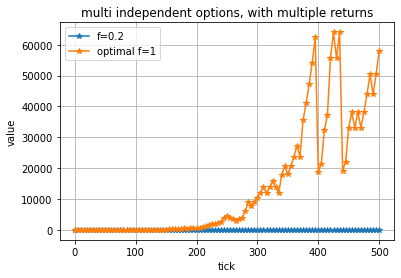
\includegraphics[width=0.9\linewidth]{single1} 
		\end{subfigure}
		\begin{subfigure}{0.525\textwidth}
			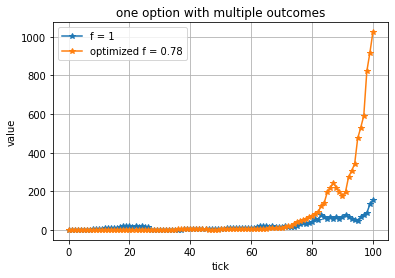
\includegraphics[width=0.9\linewidth]{single2}
		\end{subfigure}
		\begin{subfigure}{0.525\textwidth}
			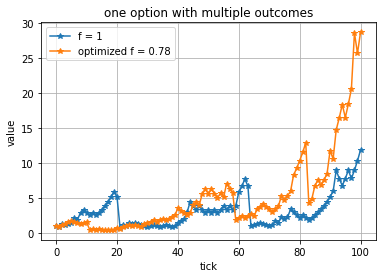
\includegraphics[width=0.9\linewidth]{single3}
		\end{subfigure}
		\begin{subfigure}{0.525\textwidth}
			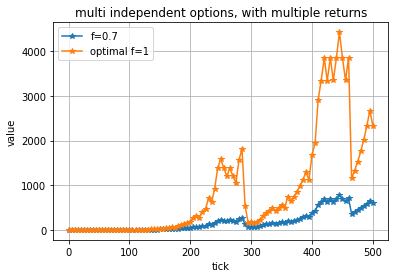
\includegraphics[width=0.9\linewidth]{single4}
		\end{subfigure}
		\caption{simulations that compare optimal fraction against random one}
		\label{Fig:single1}
	\end{figure}
	\newpage
	I tired to compile conclusions on big amount of simulations, but plotting something like histograms proved very difficult because of the big difference in the distribution between the optimal results and the regular ones.\\
	So I decided to calculate the average and the std of $1000$ simulation runs with the parameters from Table \ref{single:prob} the results are shown in Table \ref{single:results}.\\
	\begin{table}[!h]
		\centering\begin{tabular}{|c||c|c|c|c|c|}
			\hline
			\textbf{fraction:} & $0.2$ & $0.5$ & $0.6$ & $0.7$ & optimal f=$1$ \\ 
			\hline\hline
			\textbf{average:}  & $7.42$ & $149.79$ & $391.86$ & $978.19$ & $1.41 \cdot 10^4$ \\
			\hline
			\textbf{standard deviation:}  & $27.54$ & $2470.55$ & $9794.03$ & $35445.19$ & $2.58\cdot 10^6$  \\
			\hline
		\end{tabular}
		\caption{The average and standard deviation of 1000 simulation runs on different fractions}
		\label{single:results}
	\end{table}\\
	As we can clearly see the closer we got to the optimal fraction we got higher average fortune, however the deviation also got bigger.
	\newpage
	\section{The Extended Model}
	\subsection{Defining The Model}
	The new model will be very similar in some aspects to the Base model, but at the same time different and more robust. The complexity comes from the inclusion of more options with more outcomes so we will be able to calculate more realistic results. In the model each options has its own distribution of returns and our choice will not be one dimensional, but multidimensional, meaning we will need to know how to split our cash in each round.\newline
	In order to actually start talking about the returns, we will need to define our fortune at each round. in eq.\ref{multi-dim-fortune} we defined the amount of options to be $l$,  $\overrightarrow{\alpha} \in \mathbb{R}^l$ is the vector of returns ,in the vector the $i$-th element represent the return of $i$-th option, in addition the vector $\overrightarrow{f} \in \mathbb{R}^l$ represent the fractions that we invest in the options, at last the parameter $b$ represent the fraction of the money we don't invest and keep to the next round.\\
	\begin{equation}
	\label{multi-dim-fortune}
	F_N = \Bigg\{
	\begin{aligned}
		&(b + \overrightarrow{a}\cdot \overrightarrow{f})F_{N-1} &&N > 1 \text{, for each posible outcome }\overrightarrow{a}\\
		&1 &&for \enspace N=1
	\end{aligned}
	\end{equation}
	the amount of outcomes each option has is variate, meaning that the $i$-th option has $k_i$ outcomes, an outcome can be $0$ if the option didn't win at all or even negative if the loss was high enough,
	in addition if an option did win but we didn't invest in it, the value of the $i$-th element in $\overrightarrow{f}$ would be $0$ meaning it will not be taken into account in calculation of the return.
	\newline
	The only thing left to define is the probabilities in the joint distributions of the options,
	sadly finding the joint distribution is not a simple task, to produce the joint distribution from the probabilities of each option alone. Therefor from now on we will assume that the options are independent from one another in order to simplify the calculation of the joint probability, we will denote the random vector as $X$ with $l$ coordinates so that each $X_i$ would denote the $i$-th random variable corresponding the the $i$-th option inside of  $X$:
	\begin{equation}
		\label{mul-prob}
		P(X = \overrightarrow{\alpha}) = \prod_{i = 1}^l P(X_i = \alpha_i)
	\end{equation}
	After defining both the probability of each outcome (eq.\ref{mul-prob}) and the value at each round (eq.\ref{multi-dim-fortune}) we can create a working Monte-Carlo simulation, However that's not all.\\
	As before I would like to propose the big question: is there an optimal money distribution that would provide the best gains in the long run?
	Turns out, there is.\\
	In order to find such a distribution we will define a non-linear optimization problem that we would need to solve in order to find it.\\
	Looking at eq.\ref{exp:FN} as reference I would like to extend it, in order to find the gain at $\infty$ for our current model.
	\newpage
	The set $S_l$ is the Probability space:
	\[S_l = \left\{\overrightarrow{a}|\overrightarrow{a} \in \mathbb{R}^l, \text{ for every vector } \overrightarrow{a} \text{ of possible outcome for the } l \text{ options} \right\}\]
	The size of the probability space is very big because it is a Cartesian product of all the options:
	\[|S_l| = \prod_{i=1}^{l} k_l\]
	The gain function is derived from eq.\ref{exp:FN} as before making it:
	\begin{equation}
		\label{multi:gain}
		G(\overrightarrow{f}) = \lim_{N \to \infty} \frac{1}{N}\log(\frac{F_N}{F_0}) = \sum_{\overrightarrow{a} \in S_l} P(X=\overrightarrow{a})\log(b + \overrightarrow{f} \cdot \overrightarrow{a} )
	\end{equation}
	Making it a maximization problem on a simplex.
	\newline \newline
	\textbf{Maximize:} \[
		G(\overrightarrow{f}) = \sum_{\overrightarrow{a} \in S_l} P(X=\overrightarrow{a})\log(b + \overrightarrow{f} \cdot \overrightarrow{a} )
		\]
	\textbf{s.t:}
	\[
	\begin{aligned}
		&b + \sum_{i=1}^{l} f_i = 1\\
		&b\ge 0,f_i \ge 0 \text{, for } i=1..l
	\end{aligned}
	\]
	solving this NLP problem is not an easy task, which would require calculating very big system of Lagrangian multipliers, however before trying to actually solve the system I would like to make a few statements.
	\begin{thm}
		$G(f)$ (eq.\ref{multi:gain}) is a concave function in the non-negative part of $\mathbb{R}^l$.
	\end{thm}
	\begin{proof}
		In order to prove that $G(f)$ is concave, I will prove that $-G(f)$ is convex.\\
		So let's look at each component of of the sum, and prove that it is convex
		\[
		\begin{aligned}
			&&C_{\overrightarrow{a}}(f) = -\log(b + \overrightarrow{f} \cdot \overrightarrow{a})
		\end{aligned}
		\]
		because $C_{\overrightarrow{a}}(f)$ is a composition of $y(x) = -log(x)$ which is nondecreasing, univariate, convex function with a linear function, we get that the composition is convex (this property is stated as property $3$ in page $99$ inside \cite{NLP}),
		and the sum of all $C_{\overrightarrow{a}}(f)$ is convex making $-G(f)$ convex.
		\newline
	\end{proof}
	Since $G(f)$ is concave our problem is finding the maximum of a concave function, which grant us several advantages:
	\begin{enumerate}
		\item we know that a maximum point exists because of Weierstrass theorem, however because of the concavity we know that if an optimum exist inside the feasible set it is a maxima, otherwise it is somewhere in the edges of the simplex.
		\item if we use iterative algorithm that converge to a local maxima, we get that the convergence point is in fact the maxima in the constraints.
		\label{adv}
	\end{enumerate}
	Because of advantage (\ref{adv}) I decided to solve the optimization problem by using an algorithm called \textit{SLSQP}\cite{SQP}\cite{Scipy}\cite{matlab}
	(Sequential Least SQuares Programming) which aims to find a local minima in the feasible set, so I first changed the problem to a minimization problem in order to use SLSQP:
	\newline\newline
	\textbf{Minimize:} 
	 \[
	H(\overrightarrow{f}) = -\sum_{\overrightarrow{a} \in S_l} P(X=\overrightarrow{a})\log(b + \overrightarrow{f} \cdot \overrightarrow{a} )
	\]
	\textbf{s.t:}
	\[
	\begin{aligned}
		&b + \sum_{i=1}^{l} f_i = 1\\
		&b \ge 0,\text{ }f_i \ge 0 \text{, for } i=1..l
	\end{aligned}
	\]
	but because it is a convex minimization problem, which insures that the local minima is the global minima and it exists in the feasible set, which is important because SLSQP solution converges to a local minima, which in our case, would be the optimal solution.
	\newline
	Sequential Quadratic Programming that is used in SLSQP is a way to solve the KKT equations using constrained quasi-Newton methods that guarantee superlinear convergence by accumulating second-order information regarding the KKT equations, since QP subproblems are solved at each major iterations.
	\newline\newline
	It is important to note that running the SLSQP algorithm to find the optimal fraction was extremely fast, which is very assuring if this work will become the basis for an actual trading bot, which would need fast runtime in order to trade in high frequency which is very ideal according to \cite{Feng8388} and its sources.
	\subsection{Simulations Of The Extended Model}
	The new simulation holds in memory $l$ tables that represent the distribution of each option and general information like: number of rounds, $F_0$, $\overrightarrow{f}$ and $b$(fraction of the money that we don't invest). Afterwards it runs the model for the number of rounds defined at the beginning, each time picking an outcome from each of the options and calculating the amount of money at each round. At the end of the simulation it returns an array (Numpy array \cite{Numpy}) of all the results we gathered along the way.
	which I use in order to compile graphs and insights from the Monte-Carlo runs.
	The classes that generated and managed the simulations were as general as possible in order to allow flexibility with the amount of options and outcomes, which led to some difficulties when I needed to use SLSQP, because I needed to create the target function and the constraints which were very large and complicated sums and products, so in order to simplify the coding process I decided to add the $b$ parameter as the first parameter of the vector $\overrightarrow{f}$ which in a way could be described as an option with $100\%$ chance to return $100\%$ of the value (safe option), this approach helped me produce the target function as the huge sum of all the possibilities and utilize more vector operations which led to faster run-times. I used Numpy as a way to save all the relevant data together in memory to speed the simulation because it allowed for less memory reads overall.\newline
	After creating all the necessary framework and pipelines, I was able to produce a piece of software which is very flexible and able to produce as many different experiments as I wanted without the need to write a lot more code for each one of the new tests I conducted.\newline
	
	If we look at Fig (\ref{Fig:multi1}) we can see four random runs of a simulation with 3 options each with 2 outcomes, the options are described in Table \ref{table:options1}, The fractions that I used were:
	\begin{enumerate}
		\item optimal fractions from SLSQP run were: \begin{math}
			\overrightarrow{f} = 
			\begin{pmatrix}
				0 \\
				0.33 \\
				0.33 \\
				0.33 \\
			\end{pmatrix}
		\end{math}.
	\item the random fractions were: 
	\begin{math}
		\overrightarrow{f} = 
		\begin{pmatrix}
			0.6 \\
			0.2 \\
			0.2 \\
			0 
		\end{pmatrix}
	\end{math}.
	\end{enumerate}

	while Fig (\ref{Fig:multi2}) represent a bigger system of 5 options each with 3 outcomes, the options are described in Table \ref{table:options2}, and the fractions I used were:
	\begin{enumerate}
		\item optimal fractions from SLSQP run were: \begin{math}
			\overrightarrow{f} = 
			\begin{pmatrix}
				0 \\
				0.2 \\
				0.2 \\
				0.2 \\
				0.2 \\
				0.2 \\
			\end{pmatrix}
		\end{math}.
		\item the random fractions were: 
		\begin{math}
			\overrightarrow{f} = 
			\begin{pmatrix}
				0 \\
				0.5 \\
				0.5 \\
				0 \\
				0 \\
				0 \\
			\end{pmatrix}
		\end{math}.
	\end{enumerate}
	
	\newpage	
	
	\begin{table}[!h]
		\centering\begin{tabular}{|c||c|c|}
			\hline
			\textbf{probability:} & $0.7$ & $0.3$  \\ 
			\hline
			\textbf{gain} & $1.5$ & $0.4$ \\
			\hline
		\end{tabular}
		\caption{The outcomes of each option in Fig.\ref{Fig:multi1}}
		\label{table:options1}
	\end{table}
	
	\begin{figure}[!h]
		\begin{subfigure}{0.525\textwidth}
			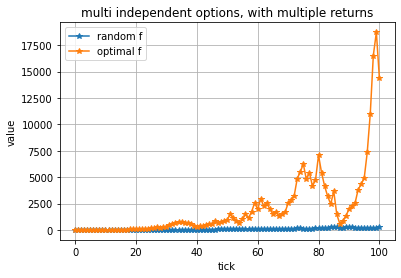
\includegraphics[width=0.9\linewidth]{multi1} 
		\end{subfigure}
		\begin{subfigure}{0.525\textwidth}
			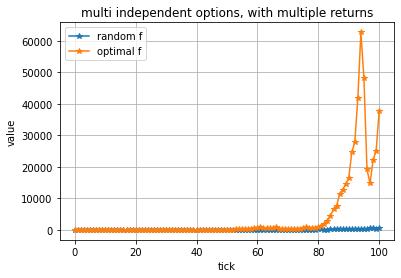
\includegraphics[width=0.9\linewidth]{multi2}
		\end{subfigure}
		\begin{subfigure}{0.525\textwidth}
			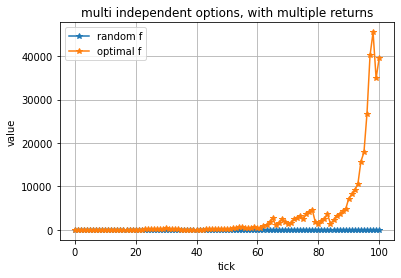
\includegraphics[width=0.9\linewidth]{multi3}
		\end{subfigure}
		\begin{subfigure}{0.525\textwidth}
			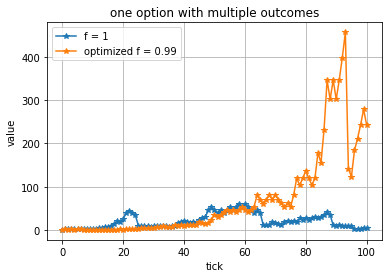
\includegraphics[width=0.9\linewidth]{multi4}
		\end{subfigure}
		\caption{Four random simulation with and without optimal value, 3 options each with 2 outcomes from Table \ref{table:options1}}
		\label{Fig:multi1}
	\end{figure}
	
		
	\begin{table}[!h]
		\centering\begin{tabular}{|c||c|c|}
			\hline
			\textbf{fraction:} & random $\overrightarrow{f}$ & optimized $\overrightarrow{f}$ \\ 
			\hline\hline
			\textbf{average:}  & $1.33\cdot 10^{12}$ & $7.45\cdot 10^{21}$ \\
			\hline
			\textbf{standard deviation:}  & $3.27\cdot 10^{13}$ & $1.53\cdot 10^{23}$ \\
			\hline
		\end{tabular}
		\caption{The average and standard deviation of 1000 simulation runs, with the data from table \ref{table:options1} and of Fig.\ref{Fig:multi1}.}
		\label{multi:results1}
	\end{table}

	\newpage
	
		\begin{table}[!h]
		\centering\begin{tabular}{|c||c|c|c|c|}
			\hline
			\textbf{probability:} & $0.15$ & $0.55$ & $0.27$ & $0.03$ \\ 
			\hline
			\textbf{gain} & $1.5$ & $1.15$ & $0.87$ & $0.3$  \\
			\hline
		\end{tabular}
		\caption{The outcomes of each option in Fig.\ref{Fig:multi2}}
		\label{table:options2}
	\end{table}
	
	
	\begin{figure}[!h]
		\begin{subfigure}{0.525\textwidth}
			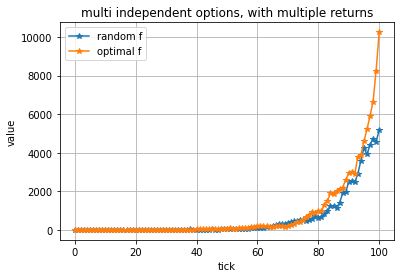
\includegraphics[width=0.9\linewidth]{multi2-1} 
		\end{subfigure}
		\begin{subfigure}{0.525\textwidth}
			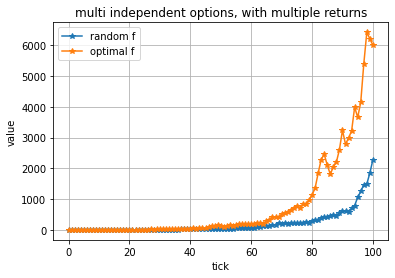
\includegraphics[width=0.9\linewidth]{multi2-2}
		\end{subfigure}
		\begin{subfigure}{0.525\textwidth}
			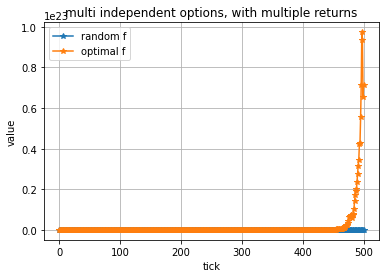
\includegraphics[width=0.9\linewidth]{multi2-3}
		\end{subfigure}
		\begin{subfigure}{0.525\textwidth}
			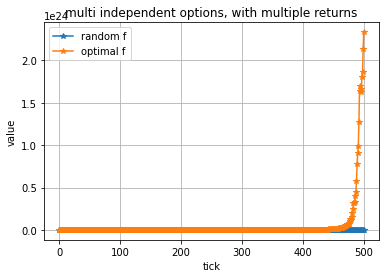
\includegraphics[width=0.9\linewidth]{multi2-4}
		\end{subfigure}
		\caption{Four random simulation with and without optimal value, 5 options each with 3 outcomes from table \ref{table:options1} and of Fig.\ref{Fig:multi1}.}
		\label{Fig:multi2}
	\end{figure}
	

	\begin{table}[!h]
		\centering\begin{tabular}{|c||c|c|}
			\hline
			\textbf{fraction:} &random $\overrightarrow{f}$ &optimized $\overrightarrow{f}$ \\
			\hline\hline
			\textbf{average:}  & $5.95\cdot 10^{15}$ & $6.84\cdot 10^{18}$ \\
			\hline
			\textbf{standard deviation:}  & $1.93\cdot 10^{17}$ & $1.54\cdot 10^{20}$ \\
			\hline
		\end{tabular}
		\caption{The average and standard deviation of 1000 simulation runs, with the data from table \ref{table:options2} and of Fig.\ref{Fig:multi2}}
		\label{multi:results2}
	\end{table}
	
	The results of both of those experiments can attest that when we take the optimal fractions our expected value grows, however our standard deviation also grows, meaning we can get wild variety of results, all of them are very high compared to the same scenarios without picking the optimal fractions
	\newpage
	
	
	
	
	\subsubsection{Example}
	let's look at the following scenario, where we have 5 options, each with the same distribution [Table \ref{prob}] (each produce $E_{gain} \ge 1$) and see what would be the best money distribution in such a scenario:\newline
	
	%% insert probability table
	\begin{table}[!h]
		\centering\begin{tabular}{|c||c|c|c|}
			\hline
			\textbf{probability:} & $0.5$ & $0.2$ & $0.3$ \\ 
			\hline
			\textbf{gain} & $1.15$ & $0.5$ & $1.5$  \\
			\hline
		\end{tabular}
	\caption{The outcomes for each option in the Fig.\ref{Fig:example1}}
	\label{prob}
	\end{table}
	
	and the optimal value we got from the SLSQP is 
	\begin{math}
		\overrightarrow{f} = 
		\begin{pmatrix}
			0 \\
			0.2 \\
			0.2 \\
			0.2 \\
			0.2 \\
			0.2 \\
		\end{pmatrix}
	\end{math}.
	\newline\newline
	Which could be surprising considering that all of the options are the same, and could have led us to believe that maybe even if had many options that are similar to each other we should have invested only in one or a couple of them, however it turns out that it's the best to stretch our investments over all of them instead of only a couple of them, in addition another interesting fact is that in-fact we don't keep any money at all and we invest all of it.\\
	\textbf{Note:} this simulation is only a single case, and more work should be put into this question in order to make an absolute statement about similar option.
		\begin{figure}[!h]
		\begin{subfigure}{0.525\textwidth}
			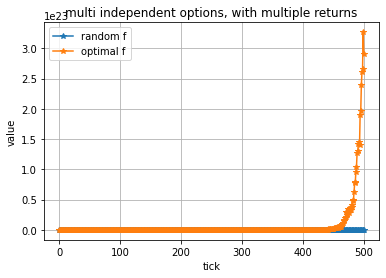
\includegraphics[width=0.9\linewidth]{example1} 
		\end{subfigure}
		\begin{subfigure}{0.525\textwidth}
			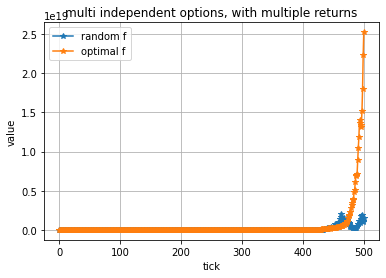
\includegraphics[width=0.9\linewidth]{example2}
		\end{subfigure}
		\caption{Two simulations for the example with random and optimal values}
		\label{Fig:example1}
	\end{figure}
	In the figure \ref{Fig:example1} the fractions we used were:
	
	\begin{enumerate}
		\item optimal fractions were: \begin{math}
			\overrightarrow{f} = 
			\begin{pmatrix}
				0 \\
				0.2 \\
				0.2 \\
				0.2 \\
				0.2 \\
				0.2 \\
			\end{pmatrix}
		\end{math}.
		\item the random fractions were: 
		\begin{math}
			\overrightarrow{f} = 
			\begin{pmatrix}
				0.0208\\
				0.5\\
				0.184\\
				0.2208\\
				0.007\\
				0.0274\\
			\end{pmatrix}
		\end{math}.
	\end{enumerate}
	
	And the results of $1000$ simulation runs:
	
	\begin{table}[!h]
		\centering\begin{tabular}{|c||c|c|}
			\hline
			\textbf{fraction:} &random $\overrightarrow{f}$ &optimized $\overrightarrow{f}$ \\
			\hline\hline
			\textbf{average:}  & $1.38\cdot 10^{18}$ & $3.21\cdot 10^{20}$ \\
			\hline
			\textbf{standard deviation:}  & $6.22\cdot 10^{19}$ & $1.59\cdot 10^{22}$ \\
			\hline
		\end{tabular}
		\caption{The average and standard deviation of $1000$ simulation runs, with the data from table \ref{prob} and of Fig.\ref{Fig:example1}}
		\label{example:results}
	\end{table}
	
	\section{Summery and conclusions}
	Kelly's criterion can be viewed as a simplified game of chance with a very powerful massage, 
	\textbf{don't on the moment and plan for the future}, the model gives us clues into the world of investments where we could sometimes win and sometimes lose, but with the ideas of mitigating losses and long term involvement, instead of looking for quick gains. We look at the long run by cutting future losses and making sure that when we lose, we won't loss all of our savings, but as a trade off when we gain we will not gain a well as we could have.\\
	When we look at the expended model we learn that splitting our money between similar investments is a good way to go, further enforcing the idea that the poor gets poorer and the rich richer, because they have much more "gas" to stretch themselves instead of just looking for quick gains. In addition the expended model at least to my own testing runs very fast which is reassuring because if this work would be the basis of a trading bot that would implement a strategy to invest in multiple options, it would be very beneficial that the bot would be fast agile, which would enable it to trade in high frequency instead of a more fundamental approach in order to maximize the gain it would have otherwise lost because of the money split, however building such a bot can be quite a hard work because we would have to download and analyze  data from many sources (like yahoo finance) and produce the joint probability for our options which can take some time and it is not an obvious work because in real world scenarios we can't assume in independency like I did in the paper, in addition Kelly's method is very strong and general meaning that if we can follow other people's investments we can use the method to determined how much money to allocate each one of them.
	\newpage
	\printbibliography[
	heading=bibintoc,
	title={References}
	]
\end{document}